\documentclass{beamer}
\usepackage[utf8]{inputenc}
\usepackage{graphicx}
\usepackage{xcolor}
\usetheme{default}
\usecolortheme{default}

\title[S03]{Section 03: Hétéroscédasticité \\ (Application Stata)}
\subtitle{GSF-6053: Économétrie Financière}
\author[SP. Boucher]{Simon-Pierre Boucher\inst{1}}
\institute[Université Laval]
{
  \inst{1}%
  Département de finance, assurance et immobilier\\
  Faculté des sciences de l'administration\\
  Université Laval}
\date[Hiver 2022]{15 février 2022}

\begin{document}

\begin{frame}
  \titlepage
\end{frame}

\begin{frame}{Application STATA}
\begin{itemize}
\item Nous allons maintenant regarder si notre régression présente un problème d’hétéroscédasticité.
\item Nous allons reprendre les mêmes données que lors de l’application STATA de la section 2.
\item Afin de détecter s’il y a présence d’hétéroscédasticité, nous allons effectuer les deux tests suivants:
\begin{itemize}
\item Test de White
\item Test de Breusch-Pagan
\end{itemize}
\end{itemize}
\end{frame}

\begin{frame}{Application STATA}
\textbf{Rappel de la régression (fait dans section 2)}
\begin{block}{Code 1: $wage = \beta_0 + \beta_1 educ +\beta_2 exper + \beta_3 tenure  + \epsilon$}
\textbf{reg wage educ exper tenure}
\end{block}

\begin{block}{Output 1:}
\begin{center}
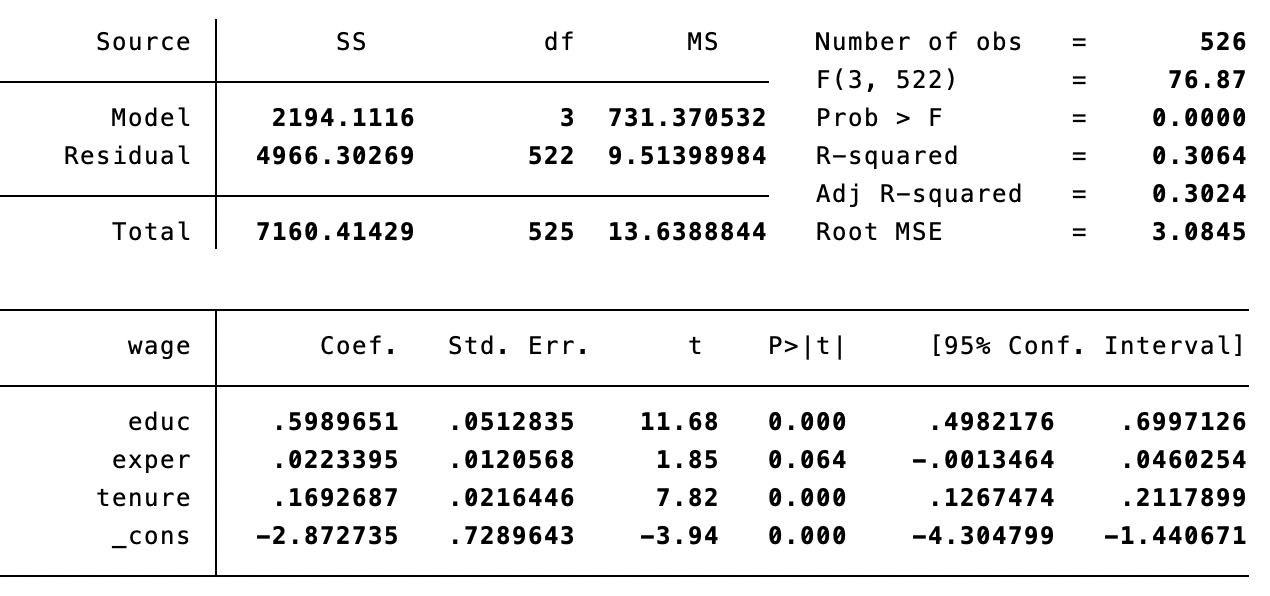
\includegraphics[scale=.5]{REG4.png}
\end{center}
\end{block}

\end{frame}

\begin{frame}{Application STATA}
\textbf{Test de White:}
\begin{itemize}
\item Régression auxiliaire:
\begin{align*}
\hat{\epsilon}^2 & = \alpha_0+\alpha_1 educ+\alpha_2 exper+\alpha_3 tenure \\ & +\alpha_{11} educ^2+\alpha_{22} exper^2  +\alpha_{33} tenure^2 \\ & +\alpha_{12}(educ \times exper) +\alpha_{13}(educ \times tenure) \\ & +\alpha_{23}(exper \times tenure) 
\end{align*}
\item La statistique de test :
\begin{align*}
WHITE = T \times R_{reg.aux}^2
\end{align*}
Sachant que $R_{reg.aux}^2$ est le $R^2$ de la régression auxiliaire.
\end{itemize}
\end{frame}

\begin{frame}{Application STATA}
\begin{block}{Code 2: Régression auxiliaire du test de White}
\begin{itemize}
 \item \textbf{predict resid, residuals}
 \item \textbf{gen resid2 = resid\string^2}
 \item \textbf{gen educ2 = educ\string^2}
 \item \textbf{gen exper2 = exper\string^2}
 \item \textbf{gen tenure2 = tenure\string^2}
 \item \textbf{gen educexper = educ*exper}
 \item \textbf{gen eductenure = educ*tenure}
 \item \textbf{gen expertenure = exper*tenure}
 \item \textbf{reg resid2 educ exper tenure educ2 exper2 tenure2 educexper eductenure expertenure}
\end{itemize}
\end{block}
\end{frame}

\begin{frame}{Application STATA}
\begin{block}{Output 2:}
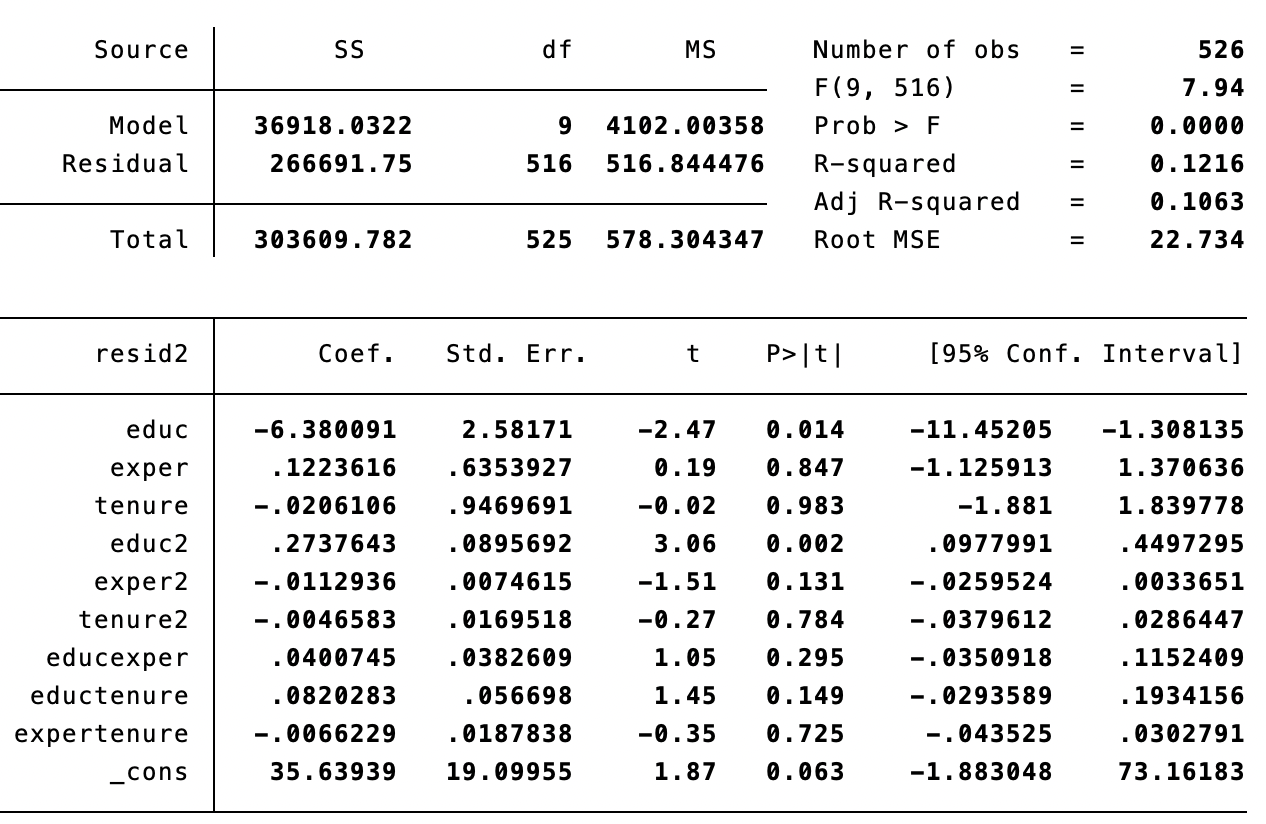
\includegraphics[scale=.5]{aux1.png}
\end{block}
\end{frame}


\begin{frame}{Application STATA}
\begin{block}{Test de White}
\begin{itemize}
\item Valeur critique de White
\begin{itemize}
\item Le nombre de degré de liberté est le nombre de variables dans la régression auxiliaire, soit $df=9$.
\item Nous trouverons cette valeur critique en utilisant une table chi-carré
\item On utilise également une significativité de 5\%
\end{itemize}
\begin{align*}
X^2(H)=X^2(9)
\end{align*}
\item Hypothèse nulle: la variance est homoscédastique
\item Hypothèse alternative: la variance est hétéroscédastique
\end{itemize}
\end{block}

\end{frame}


\begin{frame}{Application STATA}
\begin{block}{Table Chi-Carré}
\begin{center}
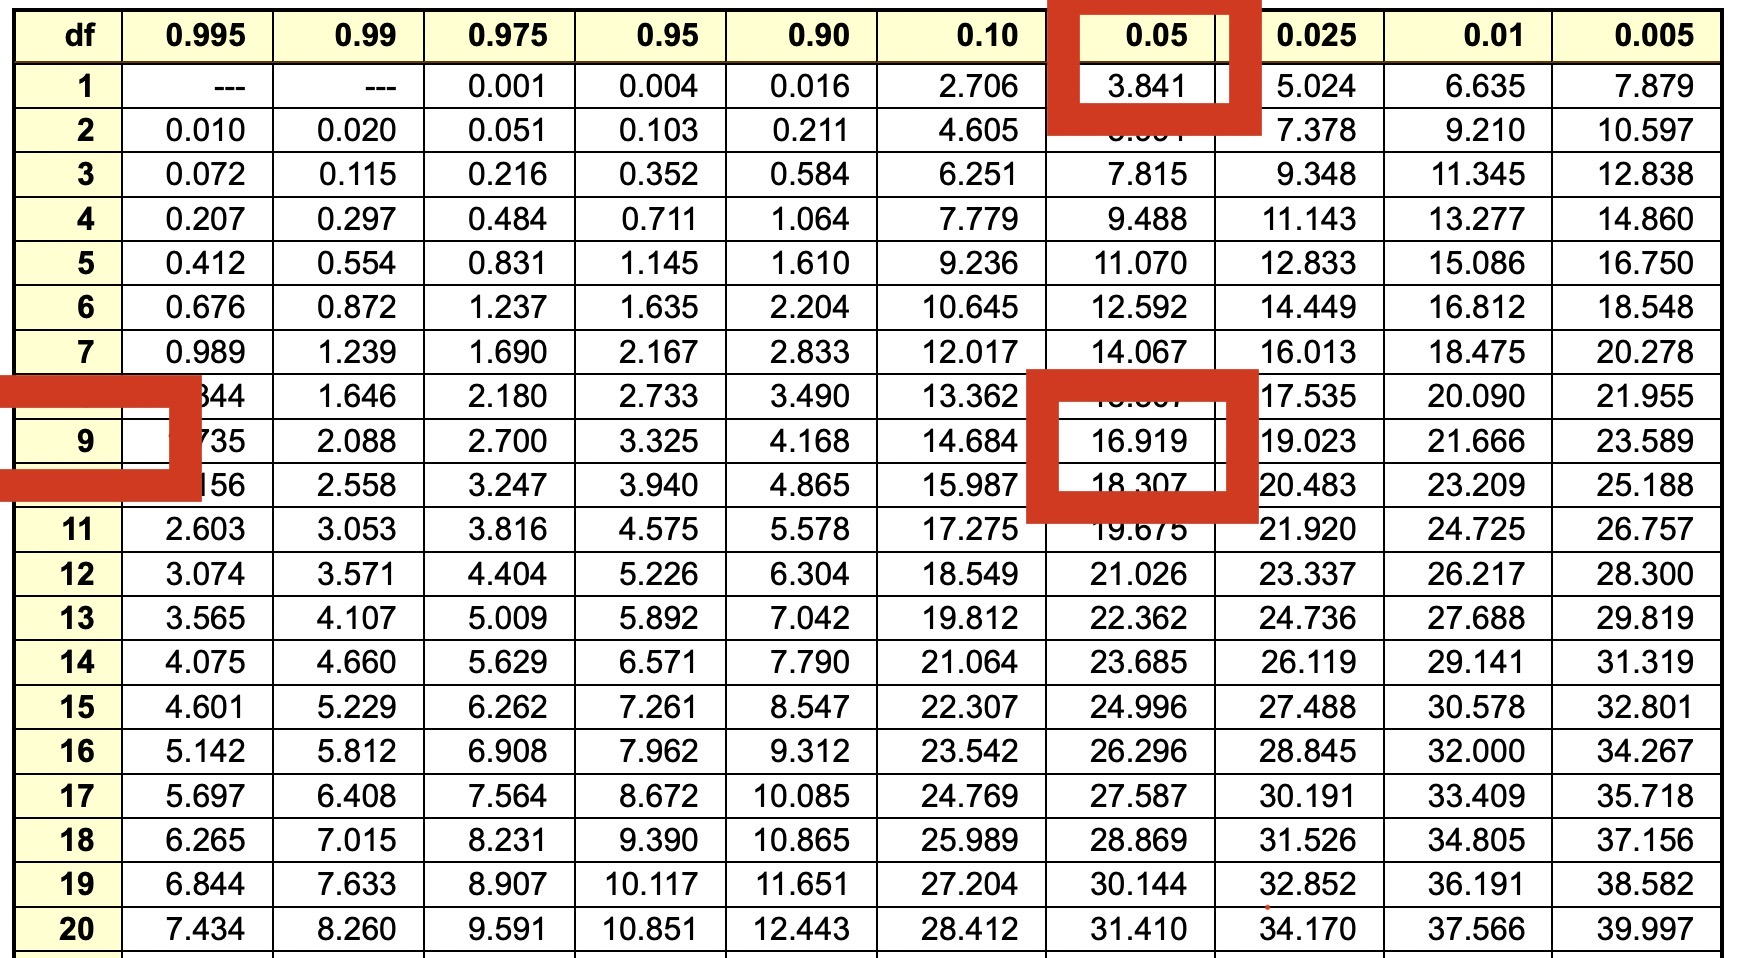
\includegraphics[scale=.17]{chitable.png}
\end{center}
\end{block}
\end{frame}


\begin{frame}{Application STATA}
\begin{block}{Valeur critique de White}
\begin{align*}
X^2(H)=X^2(9)=16.919
\end{align*}
\end{block}
\begin{block}{Statistique de White}
\begin{align*}
WHITE = T \times R_{reg.aux}^2=526 \times 0.1216 = 63.9616
\end{align*}
\end{block}

\end{frame}

\begin{frame}{Application STATA}
\begin{block}{Décision}
\begin{itemize}
\item La statistique de White $WHITE = 63.9616$ est supérieur à la valeur critique $X^2(9)=16.919$
\begin{align*}
WHITE = 63.9616 > X^2(9)=16.919
\end{align*}
\item On rejette donc l'hypothèse nulle que la variance est homoscédastique.
\item Nous avons possiblement une régression ayant une problème d'hétéroscédastique.
\end{itemize}
\end{block}
\end{frame}


\begin{frame}{Application STATA}
\begin{block}{Code 3: Test de White avec commande rapide}
\textbf{estat imtest, white}
\end{block}
\begin{block}{Output 3:}
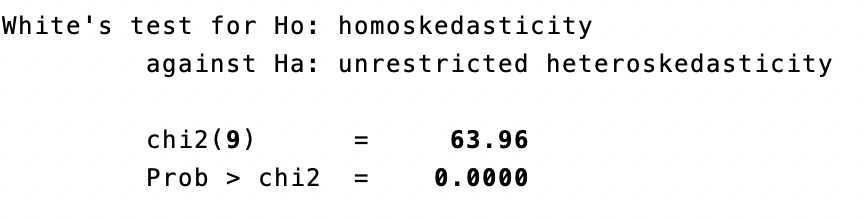
\includegraphics[scale=.5]{white.png}
\begin{itemize}
\item On peut voir que la valeur de la statistique est la même que celle obtenue avec la méthode de la régression auxiliaire.
\item Et la P-value de 0.000 confirme notre décision de rejetter l'hypthèse nulle.
\end{itemize}
\end{block}
\end{frame}


\begin{frame}{Application STATA}
\textbf{Test de Breusch-Pagan:}
\begin{itemize}
\item Régression auxiliaire:
\begin{align*}
\hat{\epsilon}^2 & = \alpha_0+\alpha_1 educ+\alpha_2 exper+\alpha_3 tenure 
\end{align*}
\item La statistique de test :
\begin{align*}
BP = T \times R_{reg.aux}^2
\end{align*}
Sachant que $R_{reg.aux}^2$ est le $R^2$ de la régression auxiliaire.
\end{itemize}
\end{frame}

\begin{frame}{Application STATA}
\begin{block}{Code 4: Régression auxiliaire du test de Breusch-Pagan}
\begin{itemize}
 \item \textbf{predict resid, residuals}
 \item \textbf{gen resid2 = resid\string^2}
 \item \textbf{reg resid2 educ exper tenure}
\end{itemize}
\end{block}
\end{frame}


\begin{frame}{Application STATA}
\begin{block}{Output 4:}
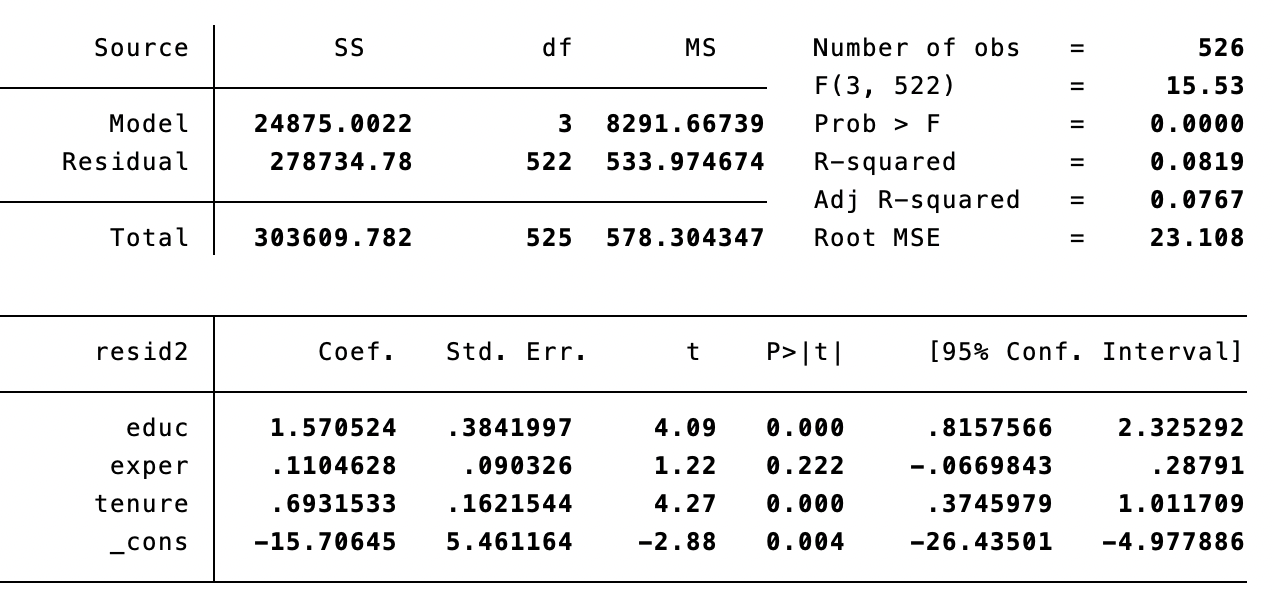
\includegraphics[scale=.5]{aux2.png}
\end{block}
\end{frame}


\begin{frame}{Application STATA}
\begin{block}{Test de Breusch-Pagan}
\begin{itemize}
\item Valeur critique de Breusch-Pagan
\begin{itemize}
\item Le nombre de degré de liberté est le nombre de variables dans la régression auxiliaire, soit $df=3$.
\item Nous trouverons cette valeur critique en utilisant une table chi-carré
\item On utilise également une significativité de 5\%
\end{itemize}
\begin{align*}
X^2(H)=X^2(3)
\end{align*}
\item Hypothèse nulle: la variance est homoscédastique
\item Hypothèse alternative: la variance est hétéroscédastique
\end{itemize}
\end{block}

\end{frame}

\begin{frame}{Application STATA}
\begin{block}{Table Chi-Carré}
\begin{center}
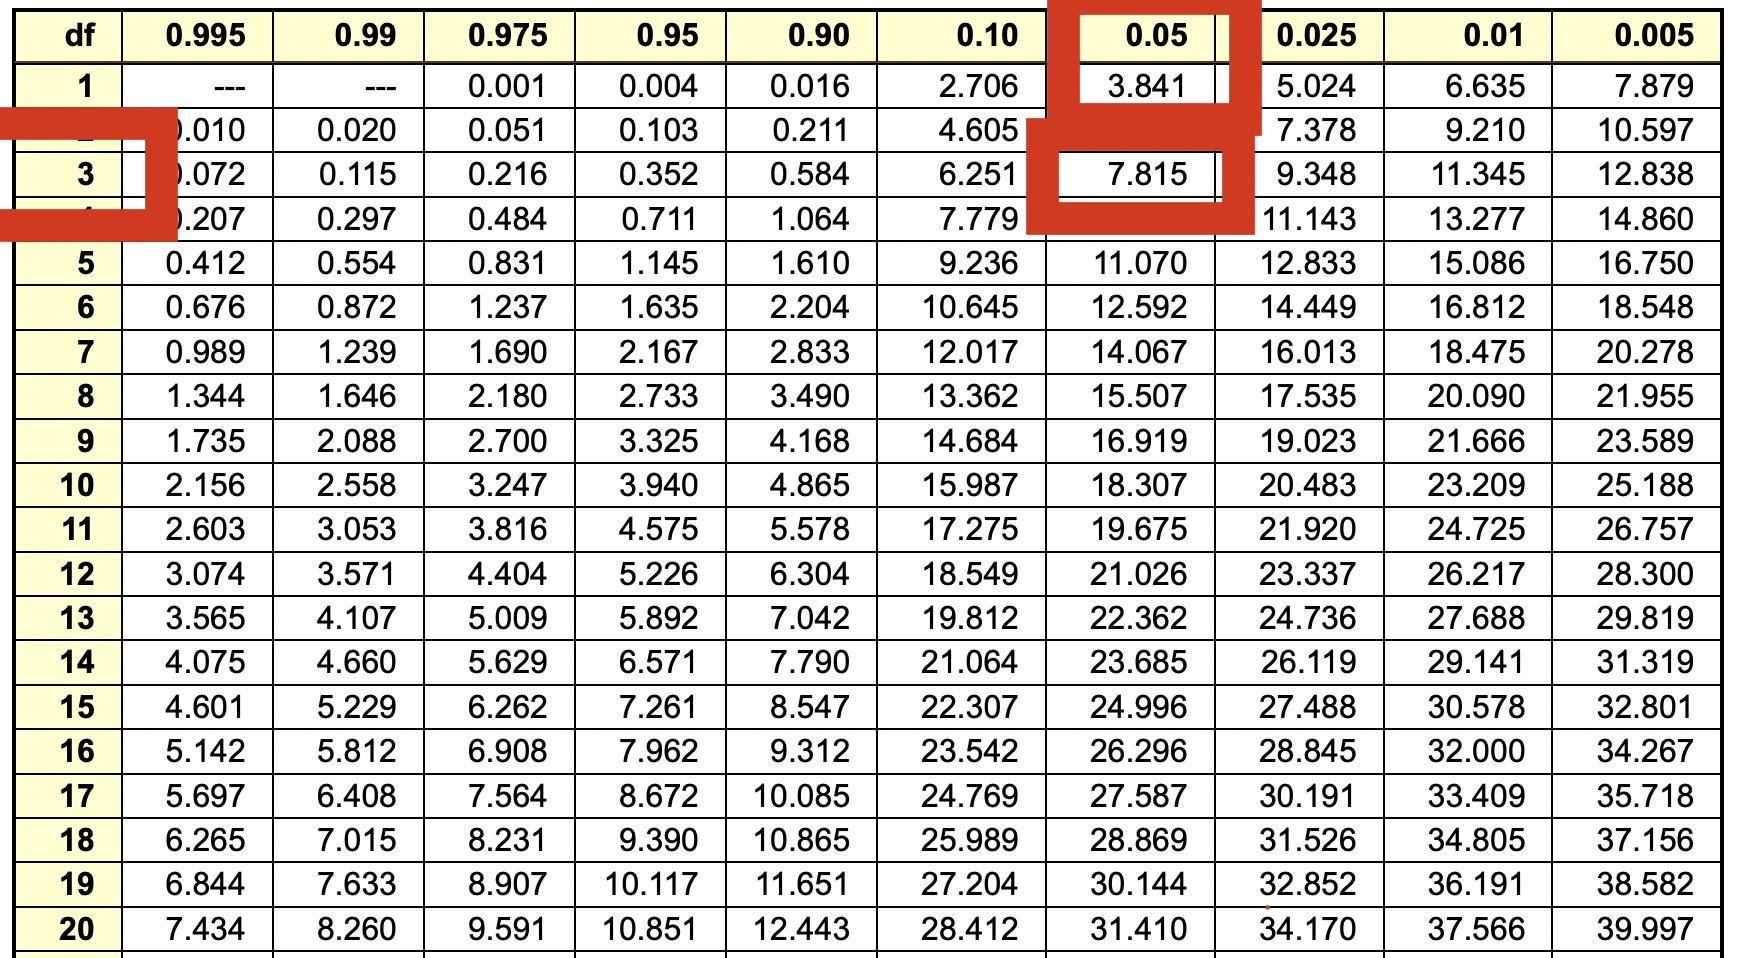
\includegraphics[scale=.17]{chitable_2.png}
\end{center}
\end{block}
\end{frame}


\begin{frame}{Application STATA}
\begin{block}{Valeur critique de Breusch-Pagan}
\begin{align*}
X^2(H)=X^2(3)=7.815
\end{align*}
\end{block}
\begin{block}{Statistique de White}
\begin{align*}
BP = T \times R_{reg.aux}^2=526 \times 0.0819 = 43.0794
\end{align*}
\end{block}

\end{frame}

\begin{frame}{Application STATA}
\begin{block}{Décision}
\begin{itemize}
\item La statistique de Breusch-Pagan $BP = 43.0794$ est supérieur à la valeur critique $X^2(9)=7.815$
\begin{align*}
BP = 43.0794 > X^2(3)=7.815
\end{align*}
\item On rejette donc l'hypothèse nulle que la variance est homoscédastique.
\item Nous avons possiblement une régression ayant une problème d'hétéroscédastique.
\end{itemize}
\end{block}
\end{frame}


\begin{frame}{Application STATA}
\begin{block}{Code 5: Test de Breusch-Pagan avec commande rapide}
\textbf{estat hettest educ exper tenure, iid}
\end{block}
\begin{block}{Output 5:}
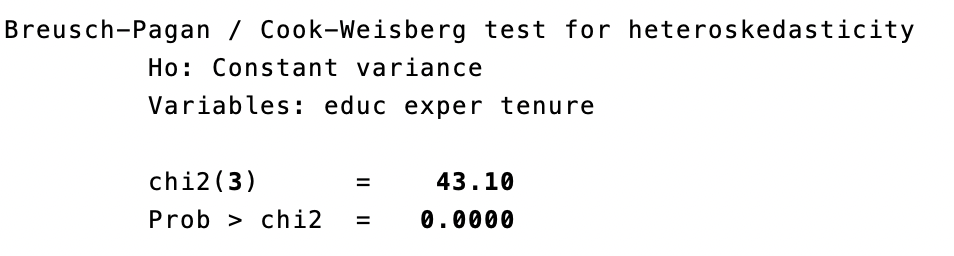
\includegraphics[scale=.5]{BP.png}
\begin{itemize}
\item On peut voir que la valeur de la statistique est la même que celle obtenue avec la méthode de la régression auxiliaire.
\item Et la P-value de 0.000 confirme notre décision de rejetter l'hypthèse nulle.
\end{itemize}
\end{block}
\end{frame}



\begin{frame}{Application STATA}
\begin{block}{Code 6: Correcteur de White \\ (Correction pour hétéroscédasticité)}
\textbf{reg wage educ exper tenure, robust}
\end{block}
\begin{block}{Output 6:}
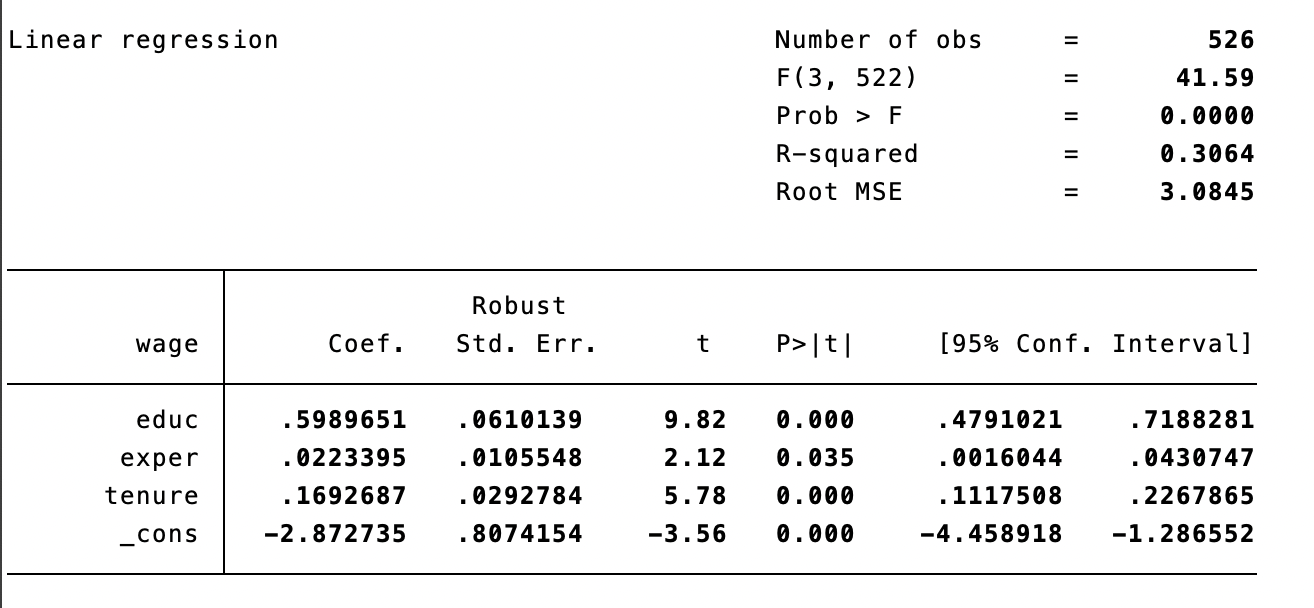
\includegraphics[scale=.5]{correcteur.png}
\end{block}
\end{frame}


\begin{frame}{Application STATA}
\begin{block}{Analyse régression corrigée pour hétéroscédasticité}
\begin{itemize}
\item Comme on peut voir, les coefficients sont restés identiques.
\item C’est normal, étant donné que le correcteur de White change simplement la variance des estimateurs et leur valeur.
\item Le fait que la variance de ses estimateurs soit affectée, implique que la décision de rejet de certains coefficients pourrait changer.
\item Les coefficients des variables \textbf{educ} et \textbf{tenure} reste significatif.
\item Cependant, dans la régression OLS, le coefficient de la variable \textbf{exper} n’était pas significatif.
\item Suite à l’application du correcteur de White, le coefficient de la variable \textbf{exper} devient significatif.
\end{itemize}
\end{block}
\end{frame}



\end{document}